\documentclass[11pt,a4paper,twoside,pdf]{article}

% Codificación y tipografía
\usepackage[T1]{fontenc}
\usepackage[utf8]{inputenc}
\usepackage{mathpazo}
\usepackage{braket}

% Matemáticas
\usepackage{amsmath, amssymb, amsfonts}
\usepackage{bm}
\usepackage[mathscr]{euscript}

% Figuras
\usepackage{graphicx}
\usepackage{float}
\usepackage{subcaption}

% Utilidades
\usepackage{multirow,rotating,array,booktabs,xspace}
\usepackage{soul,color,latexsym,xtab}

% Hipervínculos
\usepackage[colorlinks=true,urlcolor=blue,linkcolor=blue,citecolor=blue]{hyperref}

\numberwithin{equation}{section}
\usepackage[top=2.88cm,bottom=2.97cm,left=2.95cm,right=2.95cm]{geometry}

\usepackage[spanish,es-nodecimaldot,es-tabla,es-lcroman,es-nosectiondot,es-noindentfirst]{babel}
\usepackage{fancyhdr}

\newtheorem{theorem}{Teorema}[section]
\newtheorem{lemma}[theorem]{Lema}

\usepackage{listings}
\usepackage{xcolor}

\definecolor{codegreen}{rgb}{0,0.6,0}
\definecolor{codegray}{rgb}{0.5,0.5,0.5}
\definecolor{codepurple}{rgb}{0.58,0,0.82}
\definecolor{backcolour}{rgb}{0.95,0.95,0.92}

\lstdefinestyle{mystyle}{
    backgroundcolor=\color{backcolour},
    commentstyle=\color{codegreen},
    keywordstyle=\color{magenta},
    stringstyle=\color{codepurple},
    basicstyle=\ttfamily\footnotesize,
    breaklines=true, captionpos=b, keepspaces=true,
    numbers=none, showspaces=false, showstringspaces=false,
    showtabs=false, tabsize=2
}
\lstset{style=mystyle}

\linespread{1.05}

\begin{document}

% Portada %%%%%%%%%%%%%%%%%%%%%%%%%%%%%%%%%%%%%%%%%%%%%%%%%%%%%%%%%%%%%%%%%%%%%%
\pagestyle{empty}

\noindent
\begin{tabular}{r}

\includegraphics[width=8.8cm]{escudoUGRmonocromo.png} \\[-1.8ex]
\hspace{31mm}\vspace{-8mm}
\begin{tabular}{c}
\hline\\[-1ex]\hskip-2mm
{\bf Facultad de Ciencias}\hspace{18mm}
\end{tabular}
\end{tabular}

\large
\vspace{10mm}
\hspace{25mm}
\begin{tabular}{l}
Máster en Física y Matemáticas (Fisymat) \\
\end{tabular}


\vspace{5mm}
\hspace{25mm}
\begin{tabular}{l}
Análisis Numérico de EDPs y Aproximación
\\[1.5ex]
\LARGE\bf Método espectral de Galerkin\\
\LARGE\bf con polinomios de Chebyshev para\\
\LARGE\bf la ecuación de Helmholtz
\end{tabular}

\hspace{2mm}
\begin{tabular}{l}
Por:
\\
{\bf Ali-Salem Amari}\\
\end{tabular}

\begin{abstract}
Se deriva e implementa un método espectral de Galerkin con polinomios
de Chebyshev para la ecuación de Helmholtz bidimensional con
condiciones de contorno de Dirichlet homogéneas en el cuadrado
$\Omega = (-1,1)^2$. Se utiliza la base adaptada al contorno
$\phi_n(x) = T_{n+2}(x) - T_n(x)$ combinada con una construcción de
tipo producto tensorial en $\Omega$, y el sistema de Galerkin se
ensambla mediante productos de Kronecker de las matrices 1D de masa y
rigidez. Frente a una solución manufacturada suave se observa
convergencia espectral (prácticamente exponencial) hasta precisión de
máquina, un crecimiento polinómico del número de condición
$\kappa(A) \sim N^{4}$ para el Laplaciano 2D y una mejora sistemática
tanto de la precisión como del condicionamiento al aumentar el
coeficiente de reacción $k$.
\end{abstract}

% Texto %%%%%%%%%%%%%%%%%%%%%%%%%%%%%%%%%%%%%%%%%%%%%%%%%%%%%%%%%%%%%%%%%%%%%%%
\pagestyle{fancy}
\fancyhead[RO,LE]{\leftmark}
\fancyhead[LO,RE]{\thepage}
\fancyfoot{}

\newpage

\section{Planteamiento del problema}
\label{sec:intro}

Consideramos la ecuación de Helmholtz en el cuadrado
$\Omega = (-1,1)\times(-1,1)$,

\begin{equation}
\label{eq:helmholtz}
-\Delta u(x,y) + k^{2} u(x,y) = f(x,y),
\qquad (x,y) \in \Omega,
\end{equation}

con condiciones de contorno de Dirichlet homogéneas

\begin{equation}
u(x,y) = 0,
\qquad (x,y) \in \partial\Omega,
\end{equation}

y un número de onda dado $k > 0$.

Para validar el método numérico empleamos el método de soluciones
manufacturadas. Prescribimos

\begin{equation}
\label{eq:uexact}
u_{\text{exact}}(x,y) = (1-x^{2})(1-y^{2})\, e^{-x-y},
\end{equation}

que se anula en $\partial\Omega$ por construcción, y calculamos el
término fuente $f$ de forma analítica para que \eqref{eq:uexact} sea
la solución exacta de \eqref{eq:helmholtz}.

\subsection{Término fuente para la solución manufacturada}

Sea $h(x) = (1-x^{2}) e^{-x}$, de modo que
$u = h(x)\, h_{y}(y)$ con $h_{y}(y) = (1-y^{2}) e^{-y}$. Un cálculo
directo da

\begin{align*}
h'(x)  &= e^{-x}\bigl(x^{2} - 2x - 1\bigr), \\
h''(x) &= e^{-x}\bigl(-x^{2} + 4x - 1\bigr),
\end{align*}

por lo que $u_{xx} = h''(x)(1-y^{2})e^{-y}$ e igualmente para
$u_{yy}$. Reagrupando términos,

\begin{equation}
\label{eq:fsource}
\boxed{
f(x,y) = e^{-x-y}
\Bigl[
(1-y^{2})(x^{2} - 4x + 1)
+ (1-x^{2})(y^{2} - 4y + 1)
+ k^{2}(1-x^{2})(1-y^{2})
\Bigr].
}
\end{equation}

\section{Formulación débil}
\label{sec:weak}

Sea $V = H^{1}_{0}(\Omega)$. Multiplicando \eqref{eq:helmholtz} por
una función de prueba $v \in V$, integrando en $\Omega$ y aplicando
la identidad de Green con $v|_{\partial\Omega} = 0$ se obtiene el
problema variacional: hallar $u \in V$ tal que

\begin{equation}
\label{eq:weak}
a(u,v) = L(v) \qquad \forall\, v \in V,
\end{equation}

donde

\begin{align}
a(u,v) &=
\int_{\Omega} \nabla u \cdot \nabla v \; dxdy
+ k^{2} \int_{\Omega} u \, v \; dxdy,
\\[4pt]
L(v) &= \int_{\Omega} f \, v \; dxdy.
\end{align}

La forma bilineal $a(\cdot,\cdot)$ es continua y coerciva en $V$: para
todo $u \in V$,

\[
a(u,u) \;\geq\; \min(1, k^{2})\, \|u\|_{H^{1}_{0}(\Omega)}^{2}.
\]

Por el Teorema de Lax--Milgram \cite{ern2004theory} el problema tiene
solución única.

\section{Discretización espectral de Galerkin}
\label{sec:galerkin}

\subsection{Base adaptada al contorno}

Introducimos la base de Chebyshev

\begin{equation}
\phi_{n}(x) = T_{n+2}(x) - T_{n}(x),
\qquad n = 0, 1, \dots, N-1,
\end{equation}

donde $T_{n}$ es el polinomio de Chebyshev de primera especie de
grado $n$. Dado que $T_{m}(\pm 1) = (\pm 1)^{m}$, cada $\phi_{n}$
verifica

\[
\phi_{n}(\pm 1) = 0,
\]

por lo que la condición de Dirichlet está incorporada en la base
misma.  Tomamos el subespacio finito-dimensional

\[
V_{N} = \mathrm{span}\bigl\{\phi_{i}(x)\,\phi_{j}(y)
: 0 \leq i, j \leq N-1 \bigr\} \subset V.
\]

\subsection{Aproximación de Galerkin}

Buscamos la solución discreta

\begin{equation}
u_{N}(x,y) = \sum_{i=0}^{N-1}\sum_{j=0}^{N-1}
u_{ij}\, \phi_{i}(x)\,\phi_{j}(y),
\end{equation}

e imponemos \eqref{eq:weak} con cada función de prueba
$\phi_{m}(x)\phi_{n}(y)$, obteniendo

\begin{equation}
\sum_{i,j} u_{ij}\,
a\bigl(\phi_{i}\phi_{j}, \phi_{m}\phi_{n}\bigr)
= L\bigl(\phi_{m}\phi_{n}\bigr).
\end{equation}

\subsection{Ensamblaje vía productos de Kronecker}

Puesto que la base es un producto tensorial, las integrales 2D
factorizan en productos de integrales 1D:

\begin{align*}
\int_{\Omega} \nabla(\phi_{i}\phi_{j})\cdot\nabla(\phi_{m}\phi_{n}) \; dxdy
&= K_{im}\, M_{jn} + M_{im}\, K_{jn}, \\
\int_{\Omega} \phi_{i}\phi_{j}\phi_{m}\phi_{n} \; dxdy
&= M_{im}\, M_{jn},
\end{align*}

donde

\begin{equation}
M_{ij} = \int_{-1}^{1} \phi_{i}(x)\phi_{j}(x)\, dx,
\qquad
K_{ij} = \int_{-1}^{1} \phi'_{i}(x)\phi'_{j}(x)\, dx.
\end{equation}

Aplanando la matriz de coeficientes $u_{ij}$ por filas a un vector
$\mathbf{u} \in \mathbb{R}^{N^{2}}$, el sistema de Galerkin adopta la
forma compacta

\begin{equation}
\label{eq:system}
\boxed{
A\,\mathbf{u} = \mathbf{b},
\qquad
A = K \otimes M + M \otimes K + k^{2}\,(M \otimes M),
\qquad
b_{mn} = \int_{\Omega} f\,\phi_{m}\phi_{n} \; dxdy.
}
\end{equation}

Para un $N$ dado, ensamblar $A$ y $\mathbf{b}$ cuesta
$\mathcal{O}(N^{3})$, y resolver \eqref{eq:system} cuesta
$\mathcal{O}(N^{6})$ con un solver directo denso, o menos si se
explota la estructura de Kronecker.

\subsection{Cuadratura}

Las integrales 1D que definen $M$ y $K$ involucran polinomios de
grado a lo sumo $2(N+1)$; se calculan \emph{exactamente} (en
precisión de máquina) mediante una regla de Gauss--Legendre de
$N_{q} \ge N+2$ nodos \cite{canuto2006spectral}. El lado derecho
$\mathbf{b}$ emplea los mismos nodos tensorizados en $\Omega$, lo que
da la fórmula compacta

\[
b_{mn}
\;=\;
\sum_{p=1}^{N_{q}} \sum_{q=1}^{N_{q}}
w_{p}\,w_{q}\, f(x_{p},y_{q})\,\phi_{m}(x_{p})\,\phi_{n}(y_{q}).
\]

\section{Implementación en Python}
\label{sec:impl}

El núcleo del método cabe en un único módulo
\texttt{chebyshev\_core.py}. Una vez tabulada la base en los nodos de
cuadratura, $M$ y $K$ se obtienen mediante dos productos BLAS-3 y el
lado derecho mediante una sola contracción $\Phi\,F\,\Phi^{T}$.

\begin{lstlisting}[language=Python, caption={Rutinas principales de ensamblaje.}]
import numpy as np

def chebyshev_T(n, x):
    return np.cos(n * np.arccos(np.clip(x, -1.0, 1.0)))

def phi(n, x):
    return chebyshev_T(n+2, x) - chebyshev_T(n, x)

def gauss_legendre_quadrature(Nq):
    x, w = np.polynomial.legendre.leggauss(Nq)
    return x, w

def build_1D_matrices(N, Nq):
    x, w = gauss_legendre_quadrature(Nq)
    Phi  = np.vstack([phi(n, x)             for n in range(N)])
    dPhi = np.vstack([phi_derivative(n, x)  for n in range(N)])
    M = (Phi  * w) @ Phi.T
    K = (dPhi * w) @ dPhi.T
    return M, K

def build_2D_matrix(M, K, k):
    return np.kron(K, M) + np.kron(M, K) + k**2 * np.kron(M, M)

def build_rhs(N, Nq, k):
    x, w = gauss_legendre_quadrature(Nq)
    Phi  = np.vstack([phi(n, x) for n in range(N)])
    X, Y = np.meshgrid(x, x, indexing="ij")
    F    = f_source(X, Y, k)
    return ((Phi * w) @ F @ (Phi * w).T).flatten()
\end{lstlisting}

\section{Resultados numéricos}

\subsection{Solución para $N = 12$, $k = 5$}

Para el problema manufacturado, ya con $N = 12$ funciones base por
dirección se recupera la solución hasta $\sim\!10^{-13}$ en norma del
máximo.

\begin{figure}[H]
    \centering
    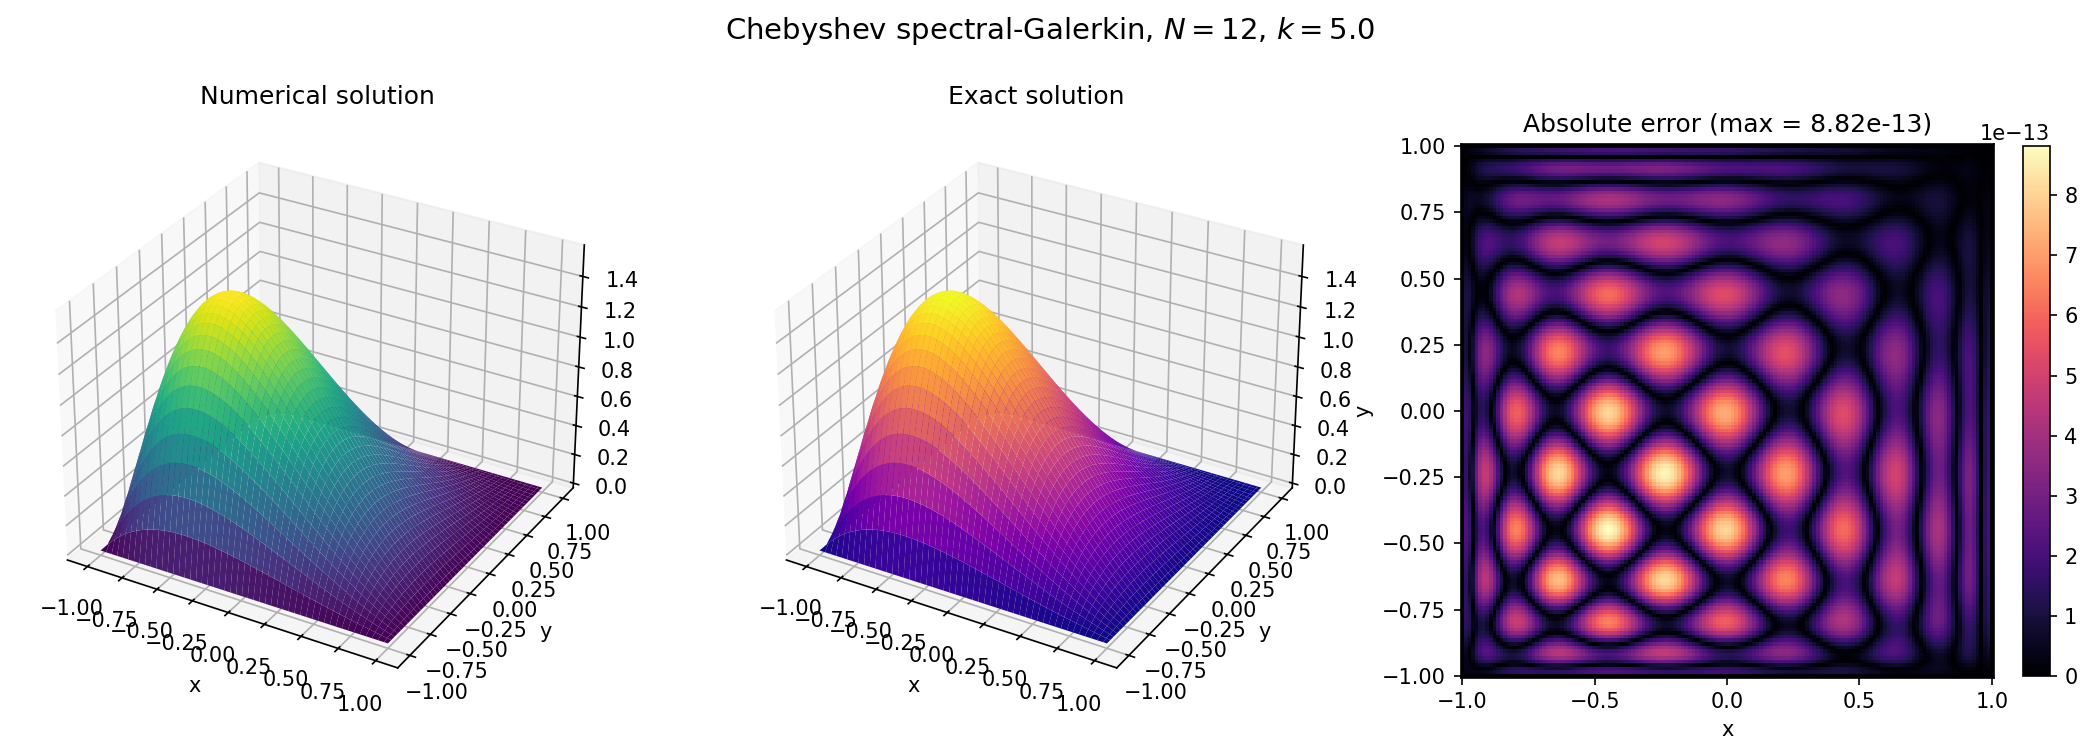
\includegraphics[width=1\linewidth]{../figures/solution.png}
    \caption{Solución numérica $u_{N}$ (izquierda), solución exacta
    $u_{\text{exact}}$ (centro) y error absoluto puntual (derecha)
    para $N = 12$, $N_{q} = 40$, $k = 5$.}
    \label{fig:solution}
\end{figure}

\subsection{Convergencia espectral}

Para la solución manufacturada suave ($C^{\infty}$), el error del
método espectral de Galerkin decae más rápido que cualquier ritmo
polinómico, saturando en la precisión de coma flotante.

\begin{figure}[H]
    \centering
    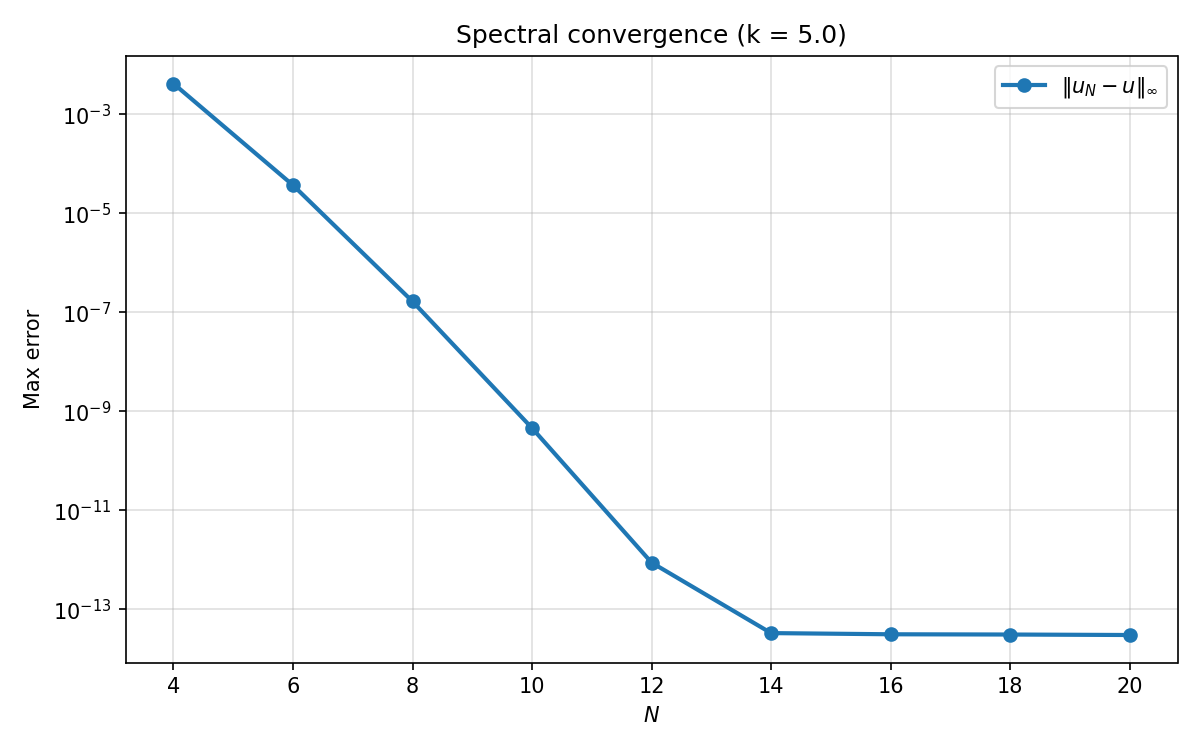
\includegraphics[width=0.8\linewidth]{../figures/convergence.png}
    \caption{Error máximo en función del tamaño $N$ de la base, en
    escala logarítmica. El error cae desde $\sim\!10^{-3}$ con $N=4$
    hasta el suelo $\mathcal{O}(10^{-14})$ para $N \ge 14$, lo que
    refleja una convergencia espectral (prácticamente exponencial).}
    \label{fig:convergence}
\end{figure}

\subsection{Número de condición}

La matriz de rigidez 2D $A$ es densa y cada vez peor condicionada al
aumentar $N$. Para la base de Chebyshev $\phi_{n} = T_{n+2} - T_{n}$
los autovalores de rigidez 1D crecen como $\mathcal{O}(n^{4})$
\cite{shen2011spectral}, y la estructura tensorial de
\eqref{eq:system} propaga el mismo ritmo $\mathcal{O}(N^{4})$ al
operador 2D.

\begin{figure}[H]
    \centering
    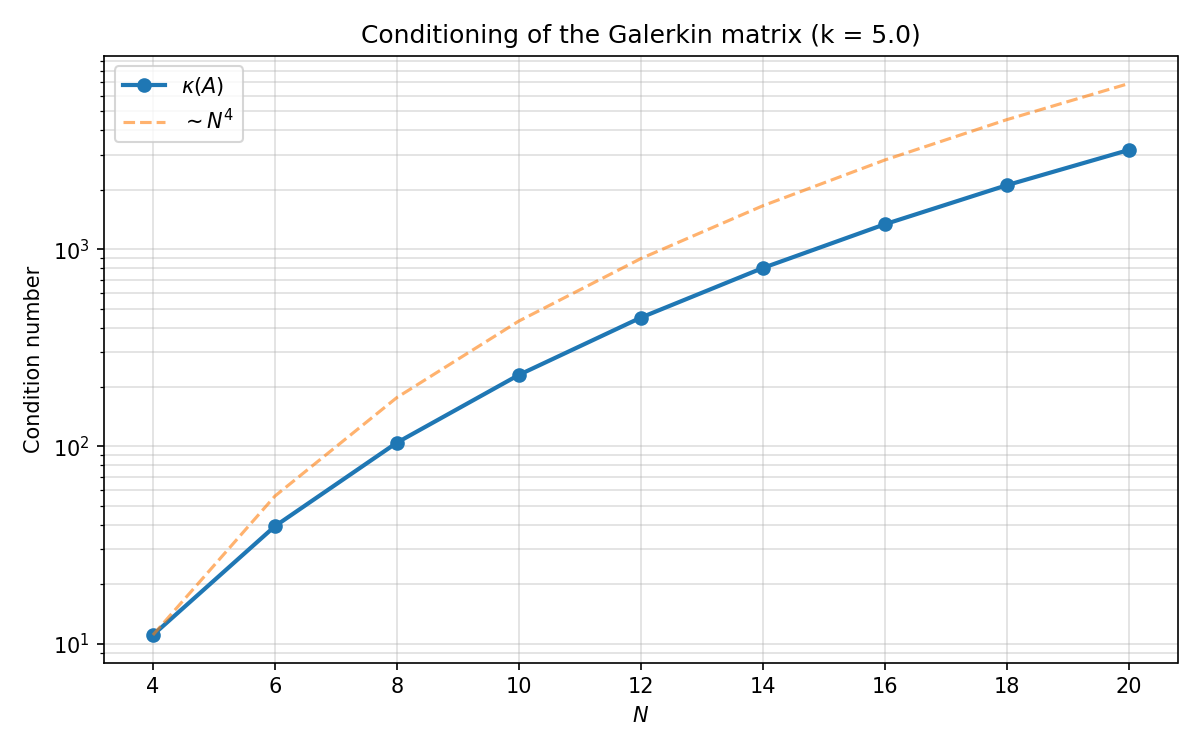
\includegraphics[width=0.8\linewidth]{../figures/condition.png}
    \caption{Número de condición $\kappa(A)$ en función de $N$ para
    $k = 5$. La línea discontinua muestra la pendiente de referencia
    $\kappa \sim N^{4}$, que ajusta bien el crecimiento medido.}
    \label{fig:condition}
\end{figure}

\subsection{Influencia del número de onda $k$}

Para esta solución manufacturada particular, suave y no oscilante,
aumentar el coeficiente de reacción $k$ refuerza la coercividad de
$a(\cdot,\cdot)$ y hace dominante la contribución de la masa en
\eqref{eq:system}. Tanto el error como el número de condición
\emph{decrecen} con $k$.

\begin{figure}[H]
    \centering
    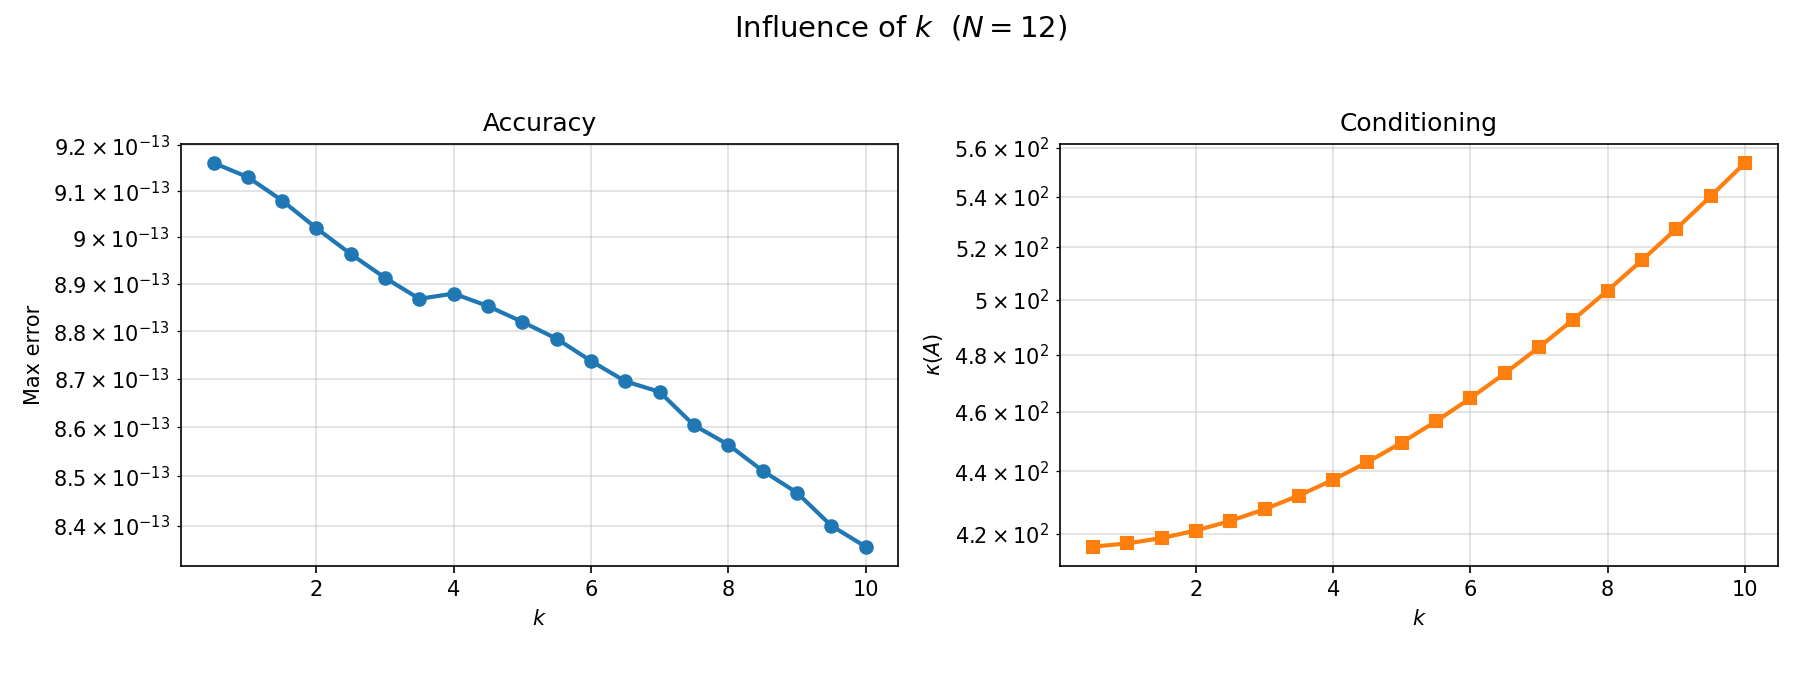
\includegraphics[width=1\linewidth]{../figures/k_influence.png}
    \caption{Precisión (izquierda) y condicionamiento (derecha) en
    función de $k$ para $N = 12$. El error baja aproximadamente un
    orden de magnitud al pasar de $k = 0.5$ a $k = 10$; el número de
    condición se reduce en un factor similar.}
    \label{fig:k_influence}
\end{figure}

\section{Conclusiones}

Se ha derivado e implementado un método espectral de Galerkin con
polinomios de Chebyshev para la ecuación de Helmholtz 2D con
condiciones de contorno de Dirichlet. La base adaptada al contorno
$\phi_{n} = T_{n+2} - T_{n}$ impone las condiciones de contorno de
manera exacta, y la construcción de tipo producto tensorial reduce
el ensamblaje 2D a tres productos de Kronecker de matrices 1D, cada
una calculada exactamente mediante cuadratura de Gauss--Legendre.
Sobre una solución manufacturada suave se ha observado

\begin{itemize}
    \item \textbf{convergencia espectral} del error máximo hasta la
          precisión de máquina para tamaños moderados $N \ge 14$;
    \item un crecimiento $\mathcal{O}(N^{4})$ del número de condición
          de la matriz de Galerkin 2D, coherente con las cotas
          clásicas para métodos de Chebyshev \cite{shen2011spectral};
    \item una ligera \emph{mejora} tanto de la precisión como del
          condicionamiento al aumentar el coeficiente de reacción $k$,
          motivada por el refuerzo de la coercividad.
\end{itemize}

Estos resultados son cualitativamente coherentes con la literatura
sobre métodos espectrales para EDPs elípticas
\cite{boyd2001chebyshev,trefethen2000spectral,canuto2006spectral}. El
mal condicionamiento intrínseco constituye la principal limitación
práctica del método en doble precisión, aunque en este proyecto
resulta aceptable porque el error satura a $10^{-13}$ bastante antes
de que $\kappa(A)$ sea problemático.

\newpage
\bibliographystyle{plain}
\bibliography{bibliography}

\end{document}
